\documentclass[a4paper,10pt]{article}
\usepackage{graphicx,wrapfig,hyperref}
\usepackage[hmargin=3.5cm,vmargin=3.0cm]{geometry}
\usepackage{glossary}
\makeglossary

% GLOSSARY
% eerst pdf maken
% dan dit uitvoeren in je terminal: makeindex requirements.glo -s requirements.ist -t requirements.glg -o requirements.gls
% dan nog een keer pdf maken

% Automatisch labelen van sections
\newcommand{\rsection}[1]{
\section{#1}\label{sec:#1}
}
\newcommand{\rsubsection}[1]{
\subsection{#1}\label{sec:sub:#1}
}
\newcommand{\rsubsubsection}[1]{
\subsubsection{#1}\label{sec:sub:sub:#1}
}

% Deze counter is voor requirements, ipv \item gebruik je \reqitem{req naam}.
% Om te referencen naar deze requirement schrijf je \reqref{req naam}.
\newcounter{rreqno}
\setcounter{rreqno}{0}
\newcommand{\rreq}[1]{\refstepcounter{rreqno}\label{#1}}
\newcommand{\reqitem}[1]{\rreq{#1}\item[(req \therreqno)]}
\newcommand{\reqref}[1]{requirement \ref{#1}}

% Use Cases
\newcommand\addrow[2]{#1 &#2\\ }

\newcommand\addheading[2]{#1 &#2\\ \hline}
\newcommand\tabularhead{\begin{tabular}{| lp{12cm} |}
\hline
}

\newcommand\addmulrow[2]{ \begin{minipage}[t][][t]{2.5cm}#1\end{minipage}% 
   &\begin{minipage}[t][][t]{8cm}
    \begin{enumerate} #2   \end{enumerate}
    \end{minipage}\\ }

\newenvironment{usecase}{\tabularhead}{\hline\end{tabular}}
% End use cases

\begin{document}

\title{TI2800 Contextproject - My Cultural Heritage\\ Requirements Analysis and Design}
\author{Sjoerd van Bekhoven\\ Tim Eversdijk \\ Herman Blanken \\ Rutger Plak \and 4014774 \\ 4005562 \\ 4078624 \\ 1358375}

\maketitle
\thispagestyle{empty}
\vspace{10cm}
\begin{figure}[ht!]
	\centering
	
\includegraphics[width=\textwidth]{cultuurapp-logo.png}
\end{figure}
\clearpage
\setcounter{page}{0}
\thispagestyle{empty}
\
\clearpage
\tableofcontents

\clearpage
\rsection{Introductie}
Het systeem \glossary{name={Systeem},description={de backend en\/of frontend}} zal toeristen \glossary{name={Toerist},description={een niet-ingelogde gebruiker van het systeem}} op een aantrekkelijke manier van zo nuttig mogelijke informatie voorzien van verschillende monumenten. Het systeem verreikt de kennis van toeristen en toont hen informatie die zij zonder het systeem niet te weten zouden zijn gekomen. Deze doelen zullen op verschillende manieren worden bereikt. De methoden die gebruikt zullen worden om deze doelen te verwezelijken staan beschreven \ref{sec:Functional requirements}.

\rsection{Overzicht}
	\rsubsection{Front-end}
\glossary{name={Front-end},description={het deel van het systeem dat zichtbaar is voor de toerist}}
	De front-end van de applicatie focust zich op twee punten:
	\begin{enumerate}
		\item Het aantrekkelijk weergeven van de informatie die we vergaard hebben van de monumenten.
		\item Het systeem zo intu\"itief mogelijk laten werken en weergeven.
	\end{enumerate}
				
	\rsubsection{Back-end}
\glossary{name={Back-end},description={het deel van het systeem dat niet zichtbaar is voor de toerist}}
	De back-end focust zich op het vergaren van nieuwe en doorgeven aan de front-end van informatie. Dit gebeurt onder andere op de volgende manieren:
	\begin{itemize}
		\item Het completeren van de database door textuele en visuele analyse.
		\item Het zoeken relevante foto's van Flickr en Wikimedia Commons.
\glossary{name={Wikimedia Commons},description={website waar miljoenen multimedia bestanden verzameld zijn, welke door iedereen vrij te gebruiken zijn}}
\glossary{name={Flickr},description={een website waarop mensen foto's kunnen uploaden en delen}}
		\item Het aanvullen van data van de monumenten door het koppelen van externe databronnen. \glossary{name={API},description={een schil die functies en data van het desbetreffende systeem beschikbaar stelt voor de buitenwereld via gedocumenteerde functies}}
		\item Het bijhouden van gebruikersinteractie en deze te gebruiken bij aanbevelingen aan toeristen.
	\end{itemize}
	
\rsection{Functional requirements}
\rsubsection{Weergaves}
	\rsubsubsection{Kaartweergave}
	\begin{enumerate}
		\reqitem{overview-maps} Het systeem moet de gefilterde monumenten (beschreven in \ref{sec:sub:Filteren en zoeken}) als spelden weergeven op een Google Maps\footnote{\label{googlemaps} http://code.google.com/apis/maps/index.html} kaart.	
		\reqitem{overview-gps} Het systeem moet de locatie van de de toerist op de Google Maps$^{\ref{googlemaps}}$ kaart aangeven, mits deze beschikbaar is. 
	\end{enumerate}
	
	\rsubsubsection{Lijstweergave} \label{sec:views-detail}
	\begin{enumerate}
		\reqitem{overview-list} De lijstweergave toont een lijst met op iedere rij een monument.
		\reqitem{overview-info} Bij ieder monument staat een thumbnail, de titel, een korte beschrijving en categorie\"en.
		\reqitem{overview-click} Wanneer de toerist op een rij klikt komt hij op de detailpagina.
\reqitem{overview-order-filter} De getoonde set monumenten wordt bepaald door de door de toerist gekozen filtering en sortering als beschreven in \ref{sec:sub:Filteren en zoeken} \& \ref{sortering}.
	\end{enumerate}
	
	\rsubsubsection{Detailpagina} \label{sec:views-detail}
	\begin{enumerate}
		\reqitem{detail-info} De detailpagina toont de naam, omschrijving, afbeelding, locatie, provincie, gemeente, stad, postcode en de categorie van het monument.
		\reqitem{detail-flickr} De detailpagina toont Flickrfoto's uit de buurt van het monument. Zie ook \ref{sec:sub:Zoeken van relevante Flickr-foto's}.
		\reqitem{detail-4sq} \label{views-checkins} De detailpagina toont het recente aantal checkins op Foursquare. Zie ook \ref{sec:sub:Foursquare}.
\glossary{name={Foursquare},description={een website waarop mensen hun locatie kunnen delen}}
		\reqitem{detail-weather} De detailpagina toont de weersverwachting rond het monument. Zie ook \ref{sec:sub:Weersinformatie}.
		\reqitem{detail-places} De detailpagina toont faciliteiten in de buurt van het monument in een kaartje. Zie ook \ref{sec:sub:Faciliteiten rond monument-locatie}.	
\reqitem{detail-places-select} De toerist heeft de mogelijkheid om te selecteren welke faciliteiten rondom de monument-locatie worden getoond.
\reqitem{detail-analyse} De detailpagina toont visueel gelijkende monumenten. Zie ook \ref{sec:sub:Monumenten vergelijken aan de hand van foto's}.
		\reqitem{detail-favorize} De detailpagina bevat een knop waarmee een CultuurApp-gebruiker het monument aan zijn favorietenlijst kan toevoegen. Zie ook \ref{sec:sub:Favorieten toevoegen}.	
\glossary{name={CultuurApp-gebruiker},description={een ingelogde gebruiker van het systeem}}
\end{enumerate}

\rsubsection{Filteren en zoeken}
\begin{enumerate}
	\reqitem{filter-distance} Toeristen kunnen monumenten filteren op een bepaalde afstand van een zoeklocatie\footnote{\label{zoeklocatie}De zoeklocatie is een tekstvak op de webpagina waar een locatie in de vorm van een adres of door google maps herkende plaatsaanduiding kan worden ingegeven. Deze kan eventueel automatisch worden ingevuld met de locatie die de browser aanbiedt.}.
	\reqitem{filter-keywords} Toeristen kunnen monumenten filteren op trefwoorden.	
	\reqitem{filter-year} Toeristen kunnen monumenten filteren op bouwjaar.
	\reqitem{filter-category} Toeristen kunnen monumenten filteren op de categorie\"en uit de dataset.
\glossary{name={Dataset},description={de set van $\sim$25.000 monumenten die is vrijgegeven voor dit project}}
	\reqitem{filter-limit} Toeristen kunnen de lengte van de lijst met monumenten limiteren. De monumenten met de hoogste sortering blijven dan staan.
\end{enumerate}
		
\rsubsection{Sortering}
\label{sortering}
\begin{enumerate}
\reqitem{sort-popularity} Toeristen kunnen monumenten sorteren op populariteit. Zie ook \ref{sec:sub:Populariteit}.
\reqitem{sort-distance} Toeristen kunnen monumenten sorteren op afstand vanaf de gegeven zoeklocatie$^{\ref{zoeklocatie}}$.
\reqitem{sort-year} Toeristen kunnen monumenten sorteren op bouwjaar.
\end{enumerate}

\rsubsection{Foursquare}
\begin{enumerate}
	\reqitem{4sq-check} Het systeem kan controleren of er voor een monument een FourSquare 'venue' (de naam van een locatie op FourSquare) bestaat.
	\reqitem{4sq-make} Het systeem kan een FourSquare venue aanmaken indien dit voor een monument nog niet bestaat.
	\reqitem{4sq-checkins} De website toont het aantal check-ins bij de venue (zie ook \reqref{views-checkins}).
	\reqitem{detail-4sq} De website slaat bij het bezoeken van de detailpagina van een monument het meest recente aantal check-ins op FourSquare op.
	\reqitem{harvest-4sq} Een beheerder kan voor een hele set toegevoegde monumenten FourSquare locaties aan laten maken en check-ins laten controleren. Dit kan ook ingepland worden.
	\glossary{name={Beheerder},description={de ontwikkelaars van de applicatie}}
\end{enumerate}
                
\rsubsection{Weersinformatie}
\begin{enumerate}
	\reqitem{harvest-weather} Er is een systeemcomponent welke live door middel van het meegeven van de longitude en latitude van een locatie de weersverwachting voor deze locatie kan ophalen van Wunderground\footnote{http://dutch.wunderground.com/weather/api/}. 
\end{enumerate}
                
\rsubsection{Faciliteiten rond monument-locatie}
\begin{enumerate}
	\reqitem{harvest-places} Er is een systeemcomponent welke door middel van het meegeven van een longitude en latitude van een locatie en een faciliteit categorie faciliteiten in de buurt van deze locatie bij Google Places kan ophalen.
\end{enumerate}
                
\rsubsection{Monumenten vergelijken aan de hand van foto's}
\begin{enumerate}
	\reqitem{analyse-online-use} Het systeem kan zoeken in de resultaten van de Visuele Analyse (zie \ref{sec:sub:Visuele analyse} om bij \'e\'en afbeelding van een monument andere afbeeldingen te vinden die visueel gelijkend zijn.
\end{enumerate}

\rsubsection{Zoeken van relevante Flickr-foto's}
\begin{enumerate}
	\reqitem{harvest-flickr} Er is een systeemcomponent dat live foto's kan ophalen van Flickr\footnote{http://www.flickr.com/services/api/} aan de hand van de geografische locatie en textuele vergelijking van tags. Zie ook \ref{sec:sub:Textuele analyse}
\end{enumerate}
			
\rsubsection{Inloggen en registreren}
Toeristen kunnen inloggen met behulp van inlogsystemen van derden. OpenID en Facebook zullen in ieder geval worden ondersteund. Dit verlaagt de drempel voor het maken van een account omdat een toerist geen extra gegevens hoeft te onthouden.
\begin{enumerate}
	\reqitem{login-fb} Een toerist kan op het systeem inloggen via hun Facebook account.
	\reqitem{login-openid} Een toerist kan op het systeem inloggen via hun OpenID account.
	\reqitem{login-capp1} Een toerist kan een eigen CultuurApp-account aanmaken op het systeem door hun email adres en een wachtwoord in te vullen.
	\reqitem{login-capp2} Een toerist kan op het systeem inloggen met hun CultuurApp-account. 
\end{enumerate}

\rsubsection{Foto's toevoegen}
De CultuurApp-gebruiker moet foto's kunnen toevoegen van een monument.
\begin{enumerate}
	\reqitem{upload} Een CultuurApp-gebruiker kan een foto uploaden naar het systeem en daarbij aangeven om welk monument het gaat
	\reqitem{upload-desc} Een CultuurApp-gebruiker kan een beschrijving meegeven aan de geuploadde foto.
	\reqitem{upload-keywords} Een CultuurApp-gebruiker kan trefwoorden meegeven aan de ge\"uploadde foto.
	\reqitem{upload-delete} Een beheerder moet een ge\"uploadde foto kunnen verwijderen uit het systeem.
\end{enumerate}

\rsubsection{Favorieten toevoegen}
\begin{enumerate}
	\reqitem{favorize-detail-favorize} Een CultuurApp-gebruiker kan monumenten toevoegen aan zijn favorietenlijst. Zie ook \reqref{detail-favorize}.
	\reqitem{defavorize} Een CultuurApp-gebruiker kan monumenten verwijderen aan zijn favorietenlijst.
	\reqitem{favorize-public} Een CultuurApp-gebruiker kan zijn favorietenlijst openbaar maken.
	\reqitem{favorize-private} Een CultuurApp-gebruiker kan zijn favorietenlijst prive maken.
\end{enumerate}

\rsubsection{Gebruikers interactie}
\begin{enumerate}
	\reqitem{harvest-interaction-information-1} Het systeem houdt voor elke toerist bij welke foto's en detail pagina's van een monument worden bekeken.
	\reqitem{harvest-interaction-information-2} Het systeem houdt voor elke toerist bij welke filter criteria worden gebruikt.
	\reqitem{link-interaction-information} Wanneer een toerist inlogt en dus een CultuurApp-gebruiker is geworden wordt de eerder verzamelde informatie ook gekoppeld aan de CultuurApp-gebruiker.
\end{enumerate}

\rsubsection{Visuele analyse}
\begin{enumerate}
	\reqitem{visuele-analyse-offline} De foto's van alle monumenten uit de dataset worden offline visueel geanalyseerd me thet programma ImageJ\footnote{http://rsbweb.nih.gov/ij/} met de plugin ImagePlot\footnote{http://lab.softwarestudies.com/p/imageplot.html}.
	\reqitem{visuele-analyse-upload} De resultaten van de offline visuele analyse worden ge\"exporteerd en ge\"upload naar de database op de webserver.
\end{enumerate}

\rsubsection{Textuele analyse}
\begin{enumerate}
 	\reqitem{text-analyse} Er is een systeemcomponent dat textuele analyse uitvoert.
 	\reqitem{text-analyse-online} Dit systeemcomponent kan teksten analyseren met Naive Bayesiaanse filters. Indien er een dienst wordt gevonden die dit kan doen (uClassify.com is een kandidaat) dan wordt deze gebruikt, zo niet dan wordt dit ge\"implementeerd.
 	\reqitem{text-analyse-thesau} Dit systeemcomponent kan lexicografisch gelijkende woorden vinden met een Thesaurus. Zie \ref{sec:sub:Thesaurus}.
\end{enumerate}
    	                
\rsubsection{Thesaurus}
\begin{enumerate}
	\reqitem{thesau} Het systeem bevat een component welke een Thesaurus bevat, bijvoorbeeld Cornetto.
	\reqitem{thesau-getter} Wanneer een component in het systeem de Thesaurus aanroept en een (lijst van) woord(en) geeft, zal een lijst van relevante woorden worden teruggegeven.
\end{enumerate}

\rsubsection{Completeren dataset}
\begin{enumerate}
	\reqitem{completing-dataset} Het systeem kan de categorie-specifieke informatie filteren uit de afbeeldingen en beschrijvingen van monumenten met behulp van visuele en textuele analyse. Zie ook \ref{sec:sub:Visuele analyse} en \ref{sec:sub:Textuele analyse}.
	\reqitem{completing-dataset-coupling} Het systeem kan met behulp van de verworven categorie-specifieke informatie de ongecategoriseerde monumenten indelen in een visueel en textueel gelijkende categorie.
\end{enumerate}

\rsubsection{Aanbevelingen}
\begin{enumerate}
	\reqitem{recom-general} Het systeem kan aanbevelingen geven aan toeristen aan de hand van het profiel dat aan de toerist of CultuurApp-gebruiker is toegewzen. Zie ook \ref{sec:sub:User profiler}.
	\reqitem{recom-general} Het systeem neemt in de aanbevelingen ook de algemene populariteit mee. Zie ook \ref{sec:sub:Populariteit}.
\end{enumerate}

\rsubsection{Populariteit}
\begin{enumerate}
	\reqitem{popularity} Het systeem kan de algemene populariteit van een monument bepalen door de volgende dingen mee te nemen in een gewogen functie:
\begin{enumerate}
\item het aantal views
\item het aantal foursquare check-ins Zie ook \ref{sec:sub:Foursquare}.
\item het aantal keer op de favorietenlijst van CultuurApp-gebruikers. Zie ook \ref{sec:sub:Favorieten toevoegen}.
	\end{enumerate}
\end{enumerate}

\rsubsection{User profiler}
\begin{enumerate}
	\reqitem{profiler-general} Het systeem kan toeristen en CultuurApp-gebruikers indelen in verschillende clusters aan de hand van handelingen van gebruikers. Zie ook \ref{sec:sub:Gebruikers interactie}.
\end{enumerate}

\rsection{Quality requirements}	
		 	 	 		
\rsubsection{Toegankelijkheid}
	\begin{enumerate}
		\reqitem{toegankelijkheid-client} De client heeft slechts een webkit of Gecko internetbrowser met een javascript engine. Dit betekent dat het op iedere computer / handheld met een gerenomeerde webbrowser (Google Chrome, Mozilla Firefox, Safari) werkt. Op een handheld device, zoals een iPhone of Android toestel, zal het systeem ook werken. 
		\reqitem{toegankelijkheid-locatie} Een toerist kan het systeem thuis gebruiken, maar ook op locatie (mits verbonden met internet).
\end{enumerate}

\rsubsection{Prestaties / Efficientie}
\begin{enumerate}	
	\reqitem{perf-js} De client berekent zelf de weergaves en de server wordt hier niet mee belast. Op deze manier wordt voorkomen dat kostbare resources worden verspilt.
\end{enumerate}

\rsubsection{Onderhoudbaarheid}
	\begin{enumerate}
		\reqitem{maint-pieces}Alle verbindingen met externe of interne data wordt aan de hand van kleine stukken code gemaakt. Deze kleine stukken code zijn eenvoudig te onderhouden.
		\reqitem{maint-repo}De updates kunnen eenvoudig op de webserver worden geinstalleerd door een nieuwe checkout van de code-repository te doen.
		\reqitem{maint-lokaal}Het lokaal ontwikkelen maakt het mogelijk nieuwe software uitvoerig te testen voor het online te zetten.
	\end{enumerate}

\rsubsection{Betrouwbaarheid en beschikbaarheid}
\begin{enumerate}
	\reqitem{avail-git} Door de manier van ontwikkelen is de server bij het updaten van de server slechts luttele seconden offline.
	\reqitem{relia-test} De betrouwbaarheid van de updates wordt gegarandeerd door de update eerst uitvoerig te testen op lokale systemen die hetzelfde zijn geconfigureerd als de webserver.
	\reqitem{avail-extern} Door het gebruik van verschillende externe databron valt bij het niet beschikbaar zijn van zo'n databron slechts (een deel van) een module uit.
	\reqitem{avail-maps} De kaarten Google Maps$^{\ref{googlemaps}}$ zijn een kritiek component, indien Google Maps niet beschikbaar is, is het systeem onbruikbaar. Google Maps heeft echter een up-time van minimaal 99,9\%\footnote{http://www.google.com/enterprise/earthmaps/maps-sla.html}. Dat komt neer op maximaal 90 seconden per dag, in de praktijk merkt een toerist hier niets van.
	\reqitem{avail-backup} Het systeem maakt elke nacht een back-up van alle opgeslagen data op een andere server.
\end{enumerate}

\rsubsection{Security} 
\begin{enumerate}
\reqitem{sec-SQL} Het framework Kohana voorkomt sql-injections wanneer queries worden geseraliseerd via dit framework.
\end{enumerate}
\rsubsection{Precisie and Accuraatheid} 
	\begin{enumerate}
		\reqitem{prec-aanbevelingen} De aanbevelingen worden door het systeem op volgorde van relevantie getoond. Wanneer toeristen consequent niet de nummer 1 aanbeveling van een monument aanklikken, zal dit betekenen dat de aanbeveling niet correct is.
\end{enumerate} 

\rsection{Design requirements}		 	 	 		
\rsubsection{Constraints based on the type of users} 
	\begin{enumerate}
		\reqitem{upload-CA-user} CultuurApp-gebruikers kunnen foto's uploaden. Zie ook \ref{sec:sub:Foto's toevoegen}.
		\reqitem{upload-tourist} Toeristen kunnen geen foto's uploaden. Zie ook \ref{sec:sub:Foto's toevoegen}.
		\reqitem{favorites-CA-user} CultuurApp-gebruikers kunnen een favorietenlijstje bijhouden. Zie ook \ref{sec:sub:Favorieten toevoegen}.
		\reqitem{favorites-tourist} Toeristen kunnen geen favorietenlijstje bijhouden. Zie ook \ref{sec:sub:Favorieten toevoegen}.
		\reqitem{recom-CA-user} CultuurApp-gebruikers krijgen recommendation gebaseerd op hun eerder verzamelde data en dus ook van voorgaande bezoeken aan het systeem. Zie ook \ref{sec:sub:Aanbevelingen}.
		\reqitem{recom-tourist} Toeristen krijgen of geen recommendation of recommendations gebaseerd op hun net verzamelde data. Zie ook \ref{sec:sub:Aanbevelingen}.
	\end{enumerate}
	
\rsection{Process requirements}	
		 	 	 		
\rsubsection{Ontwikkelingsmethode}
	\begin{enumerate}
		\reqitem{methodology} SCRUM wordt gebruikt bij het ontwikkelen van het systeem.
	\end{enumerate}
\rsubsection{Kosten en opleveringsdatum}
	\begin{enumerate}
		\reqitem{dev-enddate} Het systeem wordt 15 juni 2012 opgeleverd.
		\reqitem{dev-costs} Het systeem wordt gratis opgeleverd.
	\end{enumerate}

	\rsection{Constraints}
	\begin{enumerate}
		\reqitem{constraints-backend} De back-end van de software zal draaien op een Debian Linux machine met een Apache webserver. Visuele gelijkenissen en verschillen worden onderzocht met de objectgeori\"enteerde programmeertaal Java. De data zal worden opgeslagen in een (My)SQL database. Voor het afhandelen van verzoeken van de client wordt de programmeertaal PHP gebruikt.
		\reqitem{constraints-frontend} Aan de kant van de client wordt data opgehaald in HTML formaat. Hierin wordt de website opgebouwd met behulp van CSS. Om dynamisch dingen op de site te tonen of veranderen wordt JavaScript gebruikt.
	\end{enumerate}
		
	\clearpage
	\rsection{Analysis models}
	\rsubsection{Use case models,descriptions and scenarios}
		\rsubsubsection{Use case: monumenten zoeken}
		\begin{usecase}
		\addheading{Actor}{Toerist}
			\addrow{Doel}{De toerist kan op eenvoudige wijze monumenten zoeken aan de hand van verschillende criteria. De toerist kan aan de hand van zijn interesses de hoeveelheid monumenten verlagen zodat eenvoudig de interesses naar voren komen in de getoonde monumenten.}
			\addrow{Triggers}{De toerist maakt \'e\'en of meerdere selecties.}
			\addrow{Preconditie}{De toerist heeft een bepaalde selectie gemaakt.}
			\addrow{Stappen}{
\begin{enumerate}
\item De toerist maakt een selectie. 
\item De selectie wordt naar de server verstuurd. 
\item De data die de gebruiker heeft opgevraagd worden weergegeven aan de toerist.
\end{enumerate}}	
			\addrow{Postconditie}{De selectie van de toerist wordt omgezet naar een set monumenten die aan de selectie voldoen. In de kaartweergave zal dit betekenen dat de hoeveelheid spelden verminderd. In de lijstweergave zal dit betekenen dat de hoeveelheid informatierijen verminderd.}
			\addrow{Samenvatting}{"Als toerist wil ik aan de hand van verschillende selectiecriteria de monumenten in de resultaatpagina beperken:
				\begin{itemize}
					\item Wanneer ik kaartweergave gebruik, moeten spelden verdwijnen of verschijnen afhankelijk van of de monumenten die deze spelden verantwoorden aan deze selectiecriteria voldoen.
					\item Wanneer ik lijstweergave gebruik, moeten rijen informatie verdwijnen of verschijnen afhankelijk vam of de monumenten die deze rijen informatie verantwoorden aan deze selectiecriteria voldoen."
				\end{itemize}}
			\end{usecase}

			\rsubsubsection{Use case: Lijstweergave}
			\begin{usecase} 
			\addheading{Actor}{Toerist} 
			\addrow{Doel}{De toerist op een overzichtelijke manier van informatie over het geselecteerde monument te voorzien. De toerist moet nuttige informatie te zien krijgen. Ook moet hij informatie te zien krijgen die hem kan helpen bij het bezoeken van het monument.}
			\addrow{Triggers}{De toerist klikt op een speld op de kaart of op een rij in de lijstweergave.}
			\addrow{Preconditie}{Er is een monument geselecteerd.}
			\addrow{Postconditie}{De informatie beschreven in \ref{sec:sub:sub:Lijstweergave} wordt weergegeven.}
			\addrow{Samenvatting}{"Als toerist wil ik wanneer ik op een speld op de kaart, of informatierij in de lijstweergave klik, verwezen worden naar de pagina met informatie over het monument die de speld of informatierij verantwoord. Op deze pagina wil ik de informatie beschreven in figuur \ref{interface3} op pagina \pageref{interface3} te zien krijgen. Ik wil een kaartje te zien krijgen waarin is ingezoomd op het monument. Op de kaart worden restaurants, barretjes en andere monumenten in de buurt weergeven. Ik wil dat het systeem mijn interesses bepaald en aan de hand van mijn interesses monumenten aanraadt waar ik in ge\"interesseerd ben."}
			\end{usecase}	

			\rsubsubsection{Use case: favorieten}
			\begin{usecase} 
			\addheading{Actor}{Toerist} 
			\addrow{Doel}{De toerist kan zijn favoriete monumenten eenvoudig terugvinden.}
			\addrow{Triggers}{De toerist voegt een monument toe aan zijn favorieten.}
			\addrow{Preconditie}{De toerist heeft een interessant monument gevonden.}
			\addrow{Postconditie}{De toerist is ingelogd en heeft het monument toegevoegd aan zijn favorieten.}
			\addrow{Samenvatting}{"Als toerist wil ik wanneer ik een monument heb gevonden dat ik graag zou willen bezoeken of op een later tijdstip nogmaals wil bekijken, dat ik dit monument aan een lijst kan toevoegen. Deze lijst wil ik altijd kunnen raadplegen na inloggen met mijn gebruikersnaam/wachtwoord of een andere login-service."}
			\end{usecase}	
			
			\rsubsubsection{Use case: toevoegen foto's}
			\begin{usecase}
			\addheading{Actor}{Toerist}
\addrow{Doel}{De toerist extra foto's laten toevoegen aan de database.}
\addrow{Triggers}{De toerist upload een foto.}
			\addrow{Precondities}{De toerist heeft een foto van een monument gemaakt.}
			\addrow{Post condities}{De foto is toegevoegd aan de database van foto's die bij het monument horen.}
			\addrow{Samenvatting}{"Als toerist wil ik als ik bij een monument ben een foto kunnen maken en deze op kunnen slaan in de database. Dit wil ik doen door vanuit de mobiele applicatie een foto te maken en te uploaden. Ook kan een toerist zodra hij of zij thuis komt foto's van een monument uploaden."}
			\end{usecase}
		
\rsubsection{Business object model}
		Het "Business object model" is een globaal object model van ons systeem. Dit model is uitgebeeld in figuur \ref{bom}.
		\begin{figure}[ht!]
			\centering
			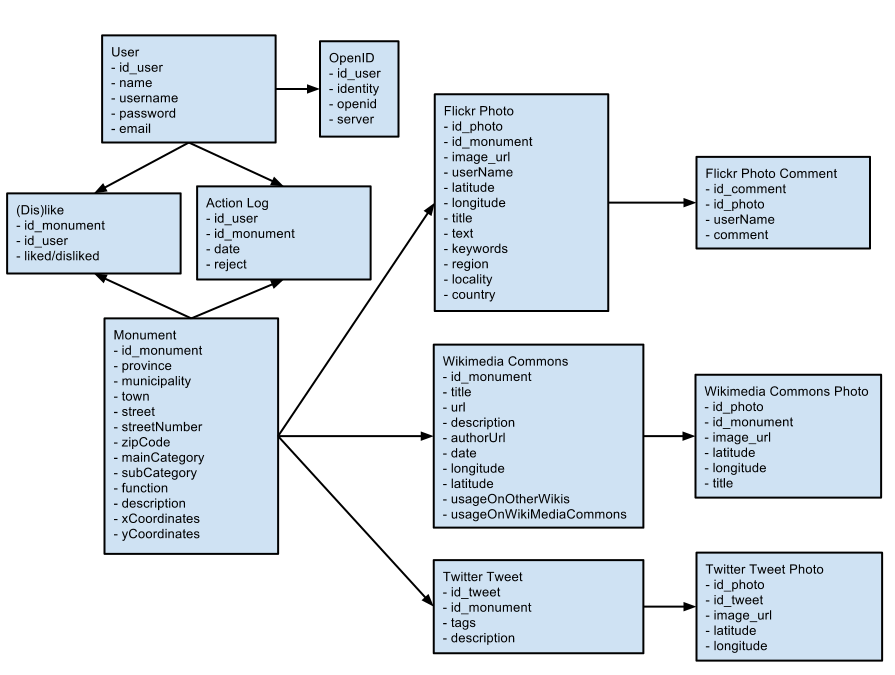
\includegraphics[width=\textwidth]{BusinessObjectModel.png}
			\caption{Business Object Model \label{bom}}
		\end{figure}
		\rsubsection{Dynamische modellen}
			\rsubsubsection{Kaartweergave}
			In figuur \ref{sequence1} is beschreven hoe de kaartweergave tot stand komt. Hierin is ook te zien hoe de informatie die op de kaart moet worden weergeven naar een externe server wordt gestuurd, waarna er een kaartje met spelden wordt teruggestuurd. Zie ook \ref{sec:sub:sub:Kaartweergave}.
\begin{figure}[ht!]
				\centering
				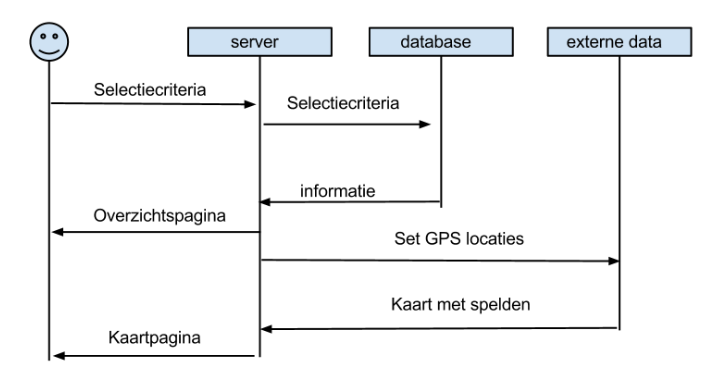
\includegraphics[width=\textwidth]{sequence1.png}
				\caption{Sequence Diagram van de lijstweergave \label{sequence1}}
			\end{figure}			

			\rsubsubsection{Detailpagina}
In figuur \ref{sequence1} is beschreven hoe de detailpagina tot stand komt. Hierin is ook te zien dat eerst het op de server beschikbare deel wordt ingeladen en daarna de informatie uit externe data-sources als deze niet zijn opgeslagen op de server. Zie ook \ref{sec:sub:sub:Detailpagina}.
			figuur \ref{sequence2}.
			\begin{figure}[ht!]
				\centering
				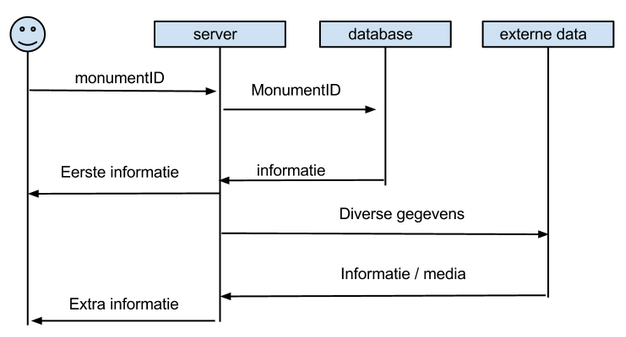
\includegraphics[width=\textwidth]{sequence2.png}
				\caption{Sequence Diagram van de detailpagina \label{sequence2}}
			\end{figure}		
		\clearpage			
		\rsection{User interface}
		In figuur \ref{interface1} is een globaal overzicht van de kaartweergave te zien, zoals beschreven in \ref{sec:sub:sub:Kaartweergave}. Hierin is duidelijk te zien hoe monumenten met speld worden aangeduid in de kaart en hoe enkele aanbevelingen worden gegeven aan de gebruiker.
			\begin{figure}[ht!]
			\centering
			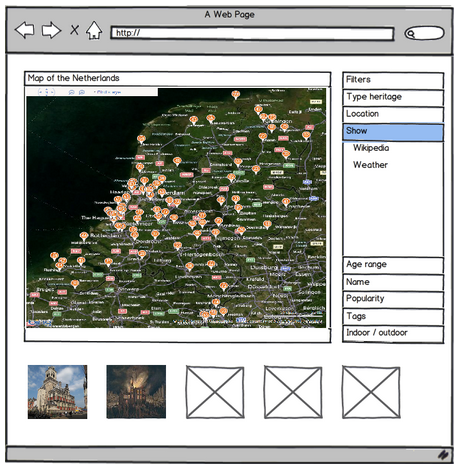
\includegraphics[height=9cm]{interface1.png}
			\caption{Globale kaartweergave \label{interface1}}
			\end{figure}
		In figuur \ref{interface2} is een globaal overzicht van de lijstweergave te zien, zoals beschreven in \ref{sec:sub:sub:Lijstweergave}. Hierin is duidelijk te zien hoe monumenten met speld worden aangeduid in de kaart en hoe enkele aanbevelingen worden gegeven aan de gebruiker.
			\begin{figure}[ht!]
				\centering
				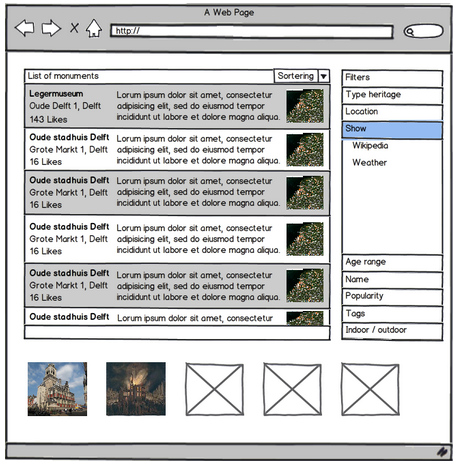
\includegraphics[height=8cm]{interface2.png}
				\caption{Globale lijstweergave \label{interface2}}
			\end{figure}
			In figuur \ref{interface3} is een globaal overzicht van de detailpagina te zien, zoals beschreven in \ref{sec:sub:sub:Detailpagina}.
			\begin{figure}[ht!]
				\centering
				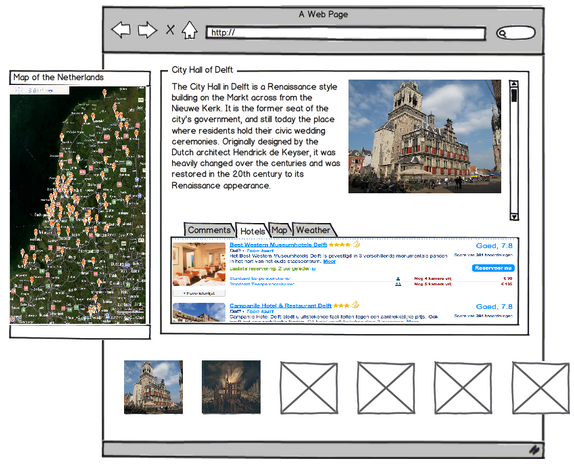
\includegraphics[height=9cm]{interface3.png}
				\caption{Globale detailpagina \label{interface3}}
			\end{figure}
	
	\clearpage

	\printglossary
\end{document}